% Created 2023-01-01 Sun 21:59
\documentclass[9pt, b5paper]{article}
\usepackage{xeCJK}
\usepackage{minted}
\usepackage[T1]{fontenc}
\usepackage[scaled]{beraserif}
\usepackage[scaled]{berasans}
\usepackage[scaled]{beramono}
\usepackage{graphicx}
\usepackage{xcolor}
\usepackage{multirow}
\usepackage{multicol}
\usepackage{float}
\usepackage{textcomp}
\usepackage{algorithm}
\usepackage{algorithmic}
\usepackage{latexsym}
\usepackage{natbib}
\usepackage{geometry}
\geometry{left=1.2cm,right=1.2cm,top=1.5cm,bottom=1.2cm}
\newminted{common-lisp}{fontsize=\footnotesize} 
\usepackage[xetex,colorlinks=true,CJKbookmarks=true,linkcolor=blue,urlcolor=blue,menucolor=blue]{hyperref}
\author{deepwaterooo}
\date{\today}
\title{手机游戏平台热更新服务器--一个实例学习笔记GeekServer}
\hypersetup{
  pdfkeywords={},
  pdfsubject={},
  pdfcreator={Emacs 27.2 (Org mode 8.2.7c)}}
\begin{document}

\maketitle
\tableofcontents


\section{手机游戏平台热更新服务器--一个实例学习笔记}
\label{sec-1}
\begin{itemize}
\item 到现在为止,基本上只找到了这一个自己可以运行的本地热更新服务器的框架.所源码基本上都读了一遍,但因为对自己来说服务器是完全陌生的领域,它读起来甚至比ET框架难多了,有不少不熟悉的概念与原理,比如Actor, TCP WebSocket等。这个框架可能学习curve会稍微陡峭一点儿,涉及到的尖端知识点比较多,比如用的是RocksDB等,很多原理自己会一一学习掌握
\item 但因为它能够运行,今天下午终于能够看进改掉visual studio 2019终端显示中文的问题.就再从运行日志入手,借助日志,把这个本地服务器弄得再明白一点儿后,准备开始着手写自己最简单的热更新服务器.
\item 这里的本地热更新服务器,与项目中游戏里的游戏客户端,接下来会需要从两端都运行,来分析学习源码.先从服务器入手
\item 今天只主要参照本地服务器的运行日志,把相对的大致步骤过程细节再补看了一遍源码.有些部分仍然不懂.
\item 明天上午会补些服务器端的基础知道,同游戏引擎客户端结合起来运行再理解消化一下这个框架
\end{itemize}
\begin{minted}[fontsize=\scriptsize,linenos=false]{text}
init NLog config...
***PolymorphicRegister Init***
2023-01-01 16:43:40.5013 INFO  launch embedded db...
2023-01-01 16:43:41.5346 INFO  regist comps...
2023-01-01 16:43:41.5346 INFO  初始化组件注册完成
2023-01-01 16:43:41.5501 INFO  load hotfix module
2023-01-01 16:43:41.5875 INFO  hotfix dll init success: F:\unityGamesExamples\GeekServer\bin\app_debug\hotfix/Geek.Server.Hotfix.dll 热更新文件地址,可以找到

// <<<<<<<<<< 我找不到下面这些是从哪里来,不知道是不是什么第三方库的.dll程序集里出来的,又或者是数据库 ? .NET Core WEB ?

// 感觉这是 TcpServer WebApplication创建时,内部生成的, 其内部创建实现原理不是很懂
2023-01-01 16:43:42.0173 DEBUG  Hosting starting 
2023-01-01 16:43:42.1014 INFO  Now listening on: http://[::]:8899
2023-01-01 16:43:42.1014 DEBUG  Loaded hosting startup assembly Geek.Server.App
2023-01-01 16:43:42.1014 INFO  Application started. Press Ctrl+C to shut down.
2023-01-01 16:43:42.1014 INFO  Hosting environment: Production
2023-01-01 16:43:42.1014 INFO  Content root path: F:\unityGamesExamples\GeekServer\bin\app_debug\
2023-01-01 16:43:42.1014 DEBUG  Hosting started
2023-01-01 16:43:42.1014 INFO  tcp 服务启动完成... 这里,这一行可以找到

// 感觉这是 HttpServer WebApplication创建时,内部生成的, 其内部创建实现原理不是很懂
2023-01-01 16:43:42.1179 DEBUG  Hosting starting
2023-01-01 16:43:42.1236 INFO  Now listening on: http://[::]:20000
2023-01-01 16:43:42.1236 DEBUG  Loaded hosting startup assembly Geek.Server.App
2023-01-01 16:43:42.1236 INFO  Application started. Press Ctrl+C to shut down.
2023-01-01 16:43:42.1236 INFO  Hosting environment: Production
2023-01-01 16:43:42.1236 INFO  Content root path: F:\unityGamesExamples\GeekServer\bin\app_debug\
2023-01-01 16:43:42.1236 DEBUG  Hosting started 

2023-01-01 16:43:42.1236 INFO  load config data // <<<<<<<<<< 这里可以找到
2023-01-01 16:43:42.2685 INFO  初始化全局定时完成
2023-01-01 16:43:42.2685 INFO  激活全局Actor: Server
2023-01-01 16:43:42.2685 INFO  下次定时回存时间 1/1/2023 4:45:05 PM
2023-01-01 16:43:42.2879 INFO  激活全局组件并检测组件是否都包含Agent实现完成

2023-01-01 16:43:42.2879 INFO  进入游戏主循环...
***进入游戏主循环***

// 下面这两行日志好像又找不到了
2023-01-01 16:43:43.6000 DEBUG  ServerCompAgent.TestSchedueTimer.延时1秒执行.每隔30秒执行
2023-01-01 16:43:45.5580 DEBUG  ServerCompAgent.TestDelayTimer.延时3秒执行.执行一次
\end{minted}
\begin{itemize}
\item 这里分两块初始化的代码主要来自于服务器热更新中的代码:
\end{itemize}
\begin{minted}[fontsize=\scriptsize,linenos=false]{csharp}
namespace Server.Logic.Common {

    internal class HotfixBridge : IHotfixBridge {
        private const string TAG = "HotfixBridge";

        private static readonly Logger Log = LogManager.GetCurrentClassLogger();
        public ServerType BridgeType => ServerType.Game;

        public async Task<bool> OnLoadSuccess(bool reload) { // 当程序集启动完成之后 的回调
            Console.WriteLine(TAG + "OnLoadSuccess() reload = " + reload);
            if (reload) {
                ActorMgr.ClearAgent();
                return true;
            }
            PolymorphicTypeMapper.Register(this.GetType().Assembly);
            HotfixMgr.SetMsgGetter(MsgFactory.GetType);

// <<<<<<<<<<<<<<<<<<<< 
            // await TcpServer.Start(Settings.TcpPort);
            await TcpServer.Start(Settings.TcpPort, builder => builder.UseConnectionHandler<AppTcpConnectionHandler>());
            Log.Info("tcp 服务启动完成...");

// <<<<<<<<<<<<<<<<<<<< 
            await HttpServer.Start(Settings.HttpPort);

// <<<<<<<<<<<<<<<<<<<< 
            Log.Info("load config data");
            (bool success, string msg) = GameDataManager.ReloadAll();
            if (!success)
                throw new Exception($"载入配置表失败... {msg}");
            GlobalTimer.Start();
            await CompRegister.ActiveGlobalComps();
            return true;
        }

        public async Task Stop() {
            // 断开所有连接
            await SessionManager.RemoveAll();
            // 取消所有未执行定时器
            await QuartzTimer.Stop();
            // 保证actor之前的任务都执行完毕
            await ActorMgr.AllFinish();
            // 关闭网络服务
            await HttpServer.Stop();
            await TcpServer.Stop();
            // 存储所有数据
            await GlobalTimer.Stop();
            await ActorMgr.RemoveAll();
        }
    }
}
\end{minted}

\section{TcpServer}
\label{sec-2}
\begin{itemize}
\item 有些是系统里的类和方法:比如下面的:
\end{itemize}
\section{IHost.cs}
\label{sec-3}

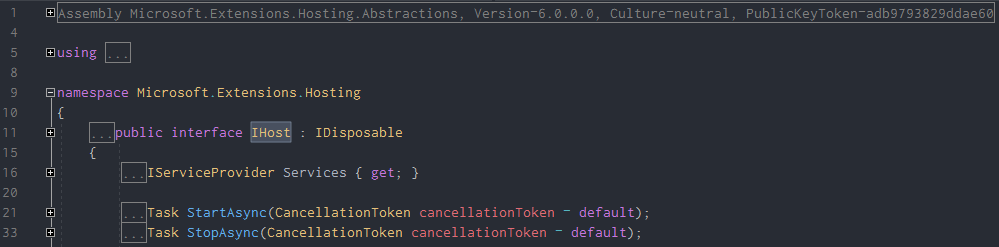
\includegraphics[width=.9\linewidth]{./pic/readme_20230101_222709.png}
\begin{itemize}
\item 这里,WebApplication的内部创建实现原理不是很懂
\end{itemize}

\section{AppStartUp: 负责服务器的启动}
\label{sec-4}
\begin{minted}[fontsize=\scriptsize,linenos=false]{csharp}
internal class AppStartUp {

    static readonly Logger Log = LogManager.GetCurrentClassLogger();

    public static async Task Enter() {
        try {
            var flag = Start(); // <<<<<<<<<<<<<<<<<<<< 
            if (!flag) return; // 启动服务器失败
            Log.Info($"launch embedded db...");
            ActorLimit.Init(ActorLimit.RuleType.None);
            GameDB.Init();
            GameDB.Open();
            Log.Info($"regist comps...");
            await CompRegister.Init();

            Log.Info($"load hotfix module");
            await HotfixMgr.LoadHotfixModule();

            Log.Info("进入游戏主循环...");
            Console.WriteLine("***进入游戏主循环***");

            Settings.LauchTime = DateTime.Now;
            Settings.AppRunning = true;
            TimeSpan delay = TimeSpan.FromSeconds(1);
            while (Settings.AppRunning) {
                await Task.Delay(delay);
            }
        }
        catch (Exception e) {
            Console.WriteLine($"服务器执行异常,e:{e}");
            Log.Fatal(e);
        }
        Console.WriteLine($"退出服务器开始");
        await HotfixMgr.Stop();
        Console.WriteLine($"退出服务器成功");
    }

    private static bool Start() { // <<<<<<<<<<<<<<<<<<<< 
        try {
            Settings.Load<AppSetting>("Configs/app_config.json", ServerType.Game); // 服务器的配置文件 

            Console.WriteLine("init NLog config..."); // 配置日志系统: CPU/IO 密集型的服务器,日志就显示狠复杂[暂放一下]
            LayoutRenderer.Register<NLogConfigurationLayoutRender>("logConfiguration");
            LogManager.Configuration = new XmlLoggingConfiguration("Configs/app_log.config");
            LogManager.AutoShutdown = false;

            PolymorphicTypeMapper.Register(typeof(AppStartUp).Assembly); // app
            PolymorphicRegister.Load();
            PolymorphicResolver.Init();
            return true;
        }
        catch (Exception e) {
            Log.Error($"启动服务器失败,异常:{e}");
            return false;
        }
    }
}
\end{minted}
\section{服务器的配置文件 Configs/app\_config.json}
\label{sec-5}

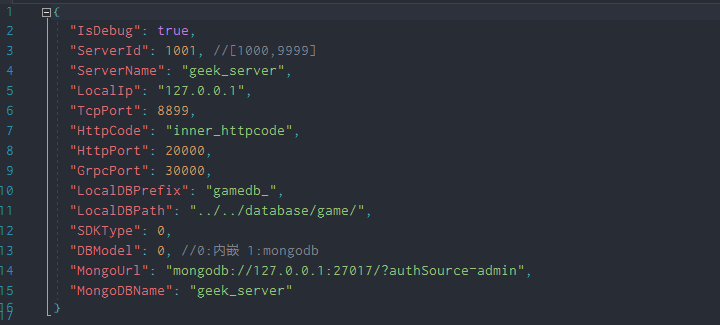
\includegraphics[width=.9\linewidth]{./pic/readme_20230101_180011.png}
\begin{minted}[fontsize=\scriptsize,linenos=false]{tex}
{
  "IsDebug": true,
  "ServerId": 1001, //[1000,9999]
  "ServerName": "geek_server",
  "LocalIp": "127.0.0.1",
  "TcpPort": 8899,
  "HttpCode": "inner_httpcode",
  "HttpPort": 20000,
  "GrpcPort": 30000,
  "LocalDBPrefix": "gamedb_",
  "LocalDBPath": "../../database/game/",
  "SDKType": 0,
  "DBModel": 0, //0:内嵌 1:mongodb
  "MongoUrl": "mongodb://127.0.0.1:27017/?authSource=admin",
  "MongoDBName": "geek_server"
}
\end{minted}
% Emacs 27.2 (Org mode 8.2.7c)
\end{document}